\section{Zielsetzung}
\label{sec:Zielsetzung}
In diesem Versuch soll die Suszeptibilität von paramagnetische Substanzen gemessen werden. 
Dazu wird von zwei Proben Seltener-Erd-Atome einmal theoretisch die Suszeptibilität berechnet und dann im Experiment mit Hilfe einer Brückenschaltung ermittelt.
Anschließend werden die Werte miteinander verglichen.
\section{Theorie}
\label{sec:Theorie}
\subsection{Berechnung der Suszeptibilität}
In Materie gilt für die magnetische Flussdichte $\vec{B}$
\begin{equation*}
    \vec{B} = \mu_0\vec{H} + \vec{M},
\end{equation*}
wobei $\mu_0$ die magnetische Feldkonstante, $\vec{H}$ die magnetische Feldstärke und $\vec{M}$ die Magnetisierung bezeichnet.
Atomare magnetische Momente lassen die Magnetisierung entstehen,welche wie folgt von $\vec{H}$ abhängt mit der Suszeptibilität $\chi$:
\begin{equation}\label{eqn:magnetisierung}
    \vec{M} = N \mu_0 \chi \vec{H} 
\end{equation}
Paramagnetismus wird von verschiedenen Orientierungen der magnetischen Momente zu einem äußeren anliegenden Feld erzeugt. 
Daher tritt er nur bei Atomen, Ionen oder Molekülen auf, die ein nicht-verschwindenden Drehimpuls haben.
Er ist grundsätzlich eine temperaturabhängige Größe, da sich durch thermisch bedingte Bewegungen die Orientierung der Momente dauerhaft ändert.\\
\\
Der Gesamtdrehimpuls $\vec{J}$ eines Atoms setzt sich zusammen aus dem Kerndrehimpuls, dem Bahndrehimpuls der Elektronenhülle $\vec{L}$ und dem Eigendrehimpuls der Elektronen (Spin) $\vec{S}$, wobei sich die letzten beiden Größen als Summe der Einzeldrehimpulse zusammensetzt.
Der Kerndrehimpuls kann für diese Betrachtung vernachlässigt werden, sodass die $LS$-Kopplung gilt: 
\begin{equation}
    \vec{J} = \vec{L} + \vec{S}
\end{equation}
Aus der Quantenmechanik ist bekannt, dass 
\begin{align}
    \vec{\mu_{\text{L}}} &= - \frac{\mu_{\text{B}}}{\hbar} \vec{L}\\
    \vec{\mu_{\text{S}}} &= - g_{\text{S}} \frac{\mu_{\text{B}}}{\hbar} \vec{S}
\end{align}
gilt, wobei $\mu_{\text{B}}$ das Bohr'sche Magneton und $g_{\text{S}}$ das gyromagnetische Verhältnis bezeichnet.
Mit der Aussage $\lvert \vec{J} \rvert = \sqrt{J(J+1)} \cdot \hbar $, welche auch analog für $\vec{S}$ und $\vec{L}$ gilt, folgt schließlich:
\begin{align}
    \lvert \vec{\mu_{\text{L}}} \rvert &= \mu_{\text{B}} \cdot \sqrt{L(L+1)} \\
    \lvert \vec{\mu_{\text{S}}} \rvert &= g_{\text{S}} \mu_{\text{B}} \cdot \sqrt{S(S+1)}
\end{align}
Bei der $LS$-Kopplung ist nur die zu $\vec{J}$ parallele oder antiparallele Komponente $\vec{\mu_{\text{J}}}$ von $\vec{\mu}$ messbar, wie die Quantenmechanik zeigt.
\begin{figure}
    \centering
    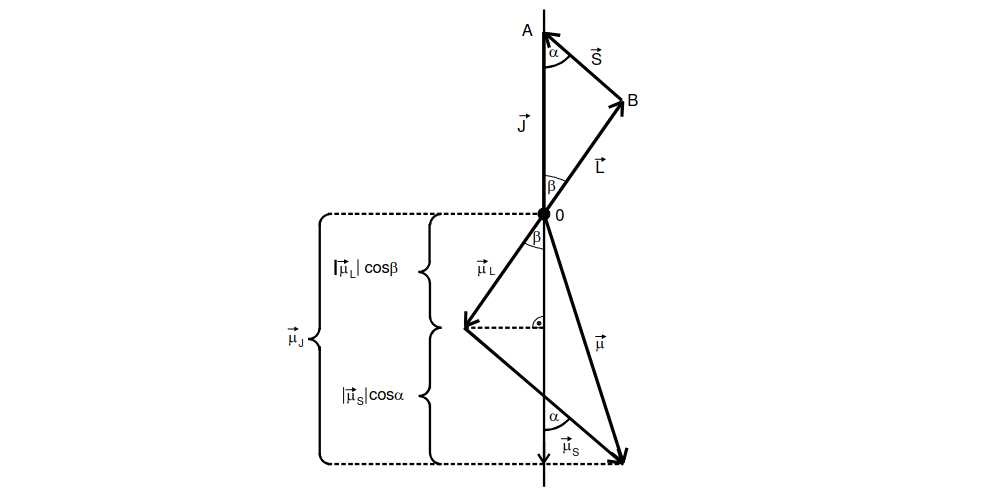
\includegraphics[width=\textwidth]{vektorielle Darstellung.png}
    \caption{Vektorielle Darstellung der Drehimpulsvektoren und deren magnetischen Momenten. \cite{anleitung}}
    \label{fig:vektoriel}
\end{figure} 
In der \autoref{fig:vektoriel} ist aus dem Vektordiagramm zu erkennen, dass
\begin{equation}
    \lvert \vec{\mu_{\text{J}}} \rvert = \lvert \vec{\mu_{\text{S}}} \rvert \cos(\alpha) + \lvert \vec{\mu_{\text{S}}} \rvert \cos(\beta)
\end{equation}
gilt, mit der Annahme das $g_{\text{S}}$ ungfähr gleich $\num{2}$ ist, vereinfacht sich der Ausdruck zu:
\begin{equation}
    \lvert \vec{\mu_{\text{J}}} \rvert \approx \mu_{\text{B}} g_{\text{J}} \sqrt{J(J+1)} 
\end{equation}
Hierbei bezeichnet $g_{\text{J}}$ den Land\'{e} - Faktor. 
\begin{equation*}
    g_{\text{J}} \coloneq \frac{3J(J+1) + S(S+1)-L(L+1)}{2J(J+1)}
\end{equation*}
Das Konzept der Richtungsquantelung aus der Quantenmechanik besagt, dass nur Winkel zwischen dem äußeren Magnetfeld und der Lage von $\vec{\mu_{\text{J}}}$ möglich, bei denen für die Z-Komponente gilt:
\begin{equation*}
    \mu_{\text{J},\text{Z}} = - \mu_{\text{B}} g_{\text{J}} m 
\end{equation*}
Das $m$ bezeichnet die Orientierungsquantenzahl, welche nur Werte von $-J$ bis $J$ annehmen kann. 
Zu jeder dieser $2J+1$ Einstellungen gibt es eine potentielle Energie über die die Magnetisierung errechnet werden kann. 
%% erklärung wie man magnetisierung bekommt
Mit Hilfe der Gleichung \eqref{eqn:magnetisierung} ist nun ein Ausdruck für die Suszeptibilität gegeben:
\begin{equation} \label{eqn:sus_theo}
    \chi = \frac{\mu_0 \mu_{\text{B}}^2 g_{\text{J}}^2 N J (J+1)}{3 k_{\text{B}} T}
\end{equation}
Hier beschreibt $k_{\text{B}}$ die Boltzmann-Konstante und $T$ die Temperatur.
Für hohe Temperaturen ergibt sich der Zusammenhang 
\begin{equation*}
    \chi \sim \frac{1}{T},
\end{equation*}
welches als Curiesche Gesetz des Paramagnetismus bekannt ist.\\
\\
Bei den zu untersuchenden Proben in diesem Versuch handelt es sich um Seltene-Erd-Atome, die durch 4f-Elektronen stark paramagnetisch sind.
Da die 4f Elektronen innerhalb der 6s-Schale liegen, sind die Ionen dieser Atome paramagnetisch.\\
Um die Werte von $J$, $S$ und $L$ herauszufinden, werden die Hund'schen Regeln und das in ihnen angesprochene Pauli-Prinzip benötigt.
Das Pauli-Prinzip sagt aus, dass sich jedes Elektron in einer Hülle in mindestens einer Quantenzahl von seinem Nachbarn unterscheiden muss.
Daraus folgt direkt, dass auf einer Schale nur endlich viele Elektronen sein können.\\
Die Hund'schen Regeln besagen, dass
\begin{enumerate}
    \item Der Gesamtspin $\vec{S}$ ist die nach dem Pauli-Prinzip maximal mögliche Summe der Einzelspins $\vec{s_{\text{i}}}$: $\vec{S} = \sum_{\text{i}} \vec{s}_{\text{i}}$.
    \item Der Drehimpuls $\vec{L}$ ist die nach der ersten Regel und dem Pauli-Prinzip maximal mögliche Summe der Bahndrehimpulse $\vec{l}_{\text{i}}$ : $\vec{L} = \sum_{\text{i}} \vec{l}_{\text{i}}$.
    \item Der Gesamtdrehimpuls $\vec{J}$ errechnet sich für eine weniger als zur Hälfte gefüllten Schale nach $\vec{J} = \vec{L} - \vec{S}$ und für einer mehr als zur Hälfte gefüllten Schale nach $\vec{J} = \vec{L} + \vec{S}$.
\end{enumerate}

\subsection{Experimentelle Ermittlung der Suszeptibilität}
Um die Suszeptibilität im Experiment zu ermitteln, wird eine Brückenschaltung nach dem Schema in \autoref{fig:Brueckenschaltung} aufgebaut.
\begin{figure}
    \centering
    \includegraphics[width=\textwidth]{Brückenschaltung.png}
    \caption{Aufbau einer Brückenschaltung zur Vermessung der paramagnetischen Substanzen \cite{anleitung}.}
    \label{fig:Brueckenschaltung}
\end{figure}
Wird die Brücke ohne Probe abgeglichen und die Brückenspannung mit einer Probe in einer der Spulen gemessen, kann die Suszeptibilität errechnet werden.
Durch die beschränkte Betrachtung von großen Frequenzen (falls $\omega^2L^2 \ll R^2$) lässt sich der Zusammenhang
\begin{equation}\label{eqn:chi_u}
    \chi_{\text{U}}(\omega\to\infty) = 4 \frac{F}{Q}\frac{U_{\text{Br}}}{U_{\text{Sp}}}
\end{equation}
zeigen, wobei $F$ der Querschnitt der Spule, $Q$ der Querschnitt der Probe und $U_{\text{Sp}}$ die Speisespannung der Brückenschaltung.\\
\\
Die Suszeptibiltät kann auch errechnet werden, wenn die Brückenschaltung mit Probe wieder abgeglichen wird und die Änderung der Widerstände notiert wird.
Aus der neuen Abgleichbedingung lässt dich die Formel 
\begin{equation}\label{eqn:chi_r}
    \chi_{\text{R}} = 2 \frac{\increment R}{R_3} \frac{F}{Q}
\end{equation}
ableiten.
Hier steht $\increment R$ für die Änderung der Widerstandes $R_3$ von den beiden abgeglichenen Zuständen.\\
Da im Experiment staubförmiges Material benutzt wird, muss der Querschnitt $Q_{\text{real}}$ ermittelt werden, welcher den Querschnitt eines Einkristalles angibt.
Aus den Formeln 
\begin{align*}
    Q_{\text{real}} &= Q \frac{\rho_{\text{p}}}{\rho_{\text{w}}}\\
    \rho_{\text{p}} &= \frac{M_{\text{p}}}{QL}
\end{align*}
lässt sich der Zusammenhang 
\begin{equation}\label{eqn:qreal}
    Q_{\text{real}} = \frac{M_{\text{p}}}{L \rho_{\text{w}}}
\end{equation}
angeben.
Hierbei beschreibt $M_{\text{p}}$ die Masse der Probe, $L$ ihre Länge und $\rho_{\text{x}}$ die Dichte der Probe ($x=p$) und des Einkristalles ($x=w$).

\subsection{Selektivverstärker}
\begin{figure}
    \centering
    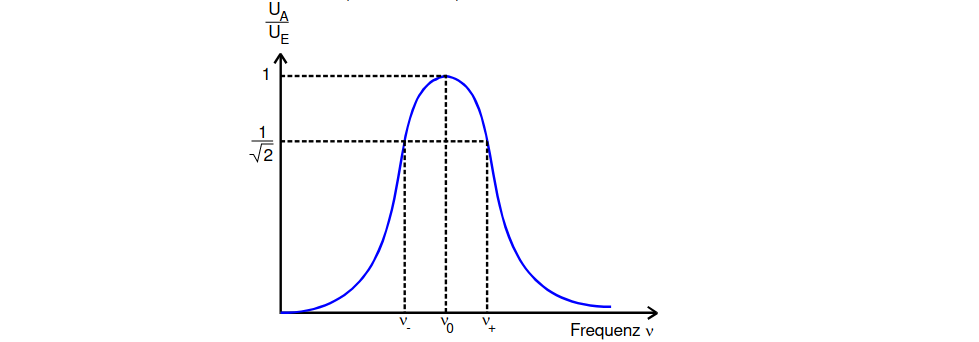
\includegraphics[width=\textwidth]{filterkurve.png}
    \caption{Die Filterkurve eines Selektivversstärkers.\cite{anleitung}}
    \label{fig:selektiv}
\end{figure}
Damit die Brückenspannung nicht unter den Störungen an den Ausgangsklemmen der Brückenschaltung verloren geht, wird das Signal verstärkt und gefiltert.
Da die Eingangsspannung der Brücke monofrequent ist, kann ein Selektivverstärker benutzt werden. 
Dies ist ein Gerät mit glockenförmiger Filterkurve, wie in der \autoref{fig:selektiv} zu sehen ist.
Die Güte $Q$ eines Selektivverstärkers ist ein Maß seiner Qualität, welche über 
\begin{equation*}
    Q = \frac{\nu_0}{\nu_+ - \nu_-}
\end{equation*}
gegeben ist, wobei $\nu_+$ bzw $\nu_-$ die Frequenzen beschreiben, wo das Verhältnis $\frac{U_{\text{A}}}{U_{\text{E}}} $ = $\frac{1}{\sqrt{2}}$ ist.
$\nu_0$ beschreibt die sogenannte Durchlassfrequenz, also die Frequenz, die am wenigsten unterdrückt wird.